
\chapter
{The PEBL Launcher}

The PEBL Launcher is the best way to navigate and launch PEBL
experiments, especially for novices or research assistants.  It allows
one to specify a few specific options that are frequently changed,
navigate through the PEBL Test Battery, and create and save
'experiment chains' to let you run multiple experiments in a row.

\begin{figure}[h]
\caption{Screenshot of of PEBL Launcher.}
\center
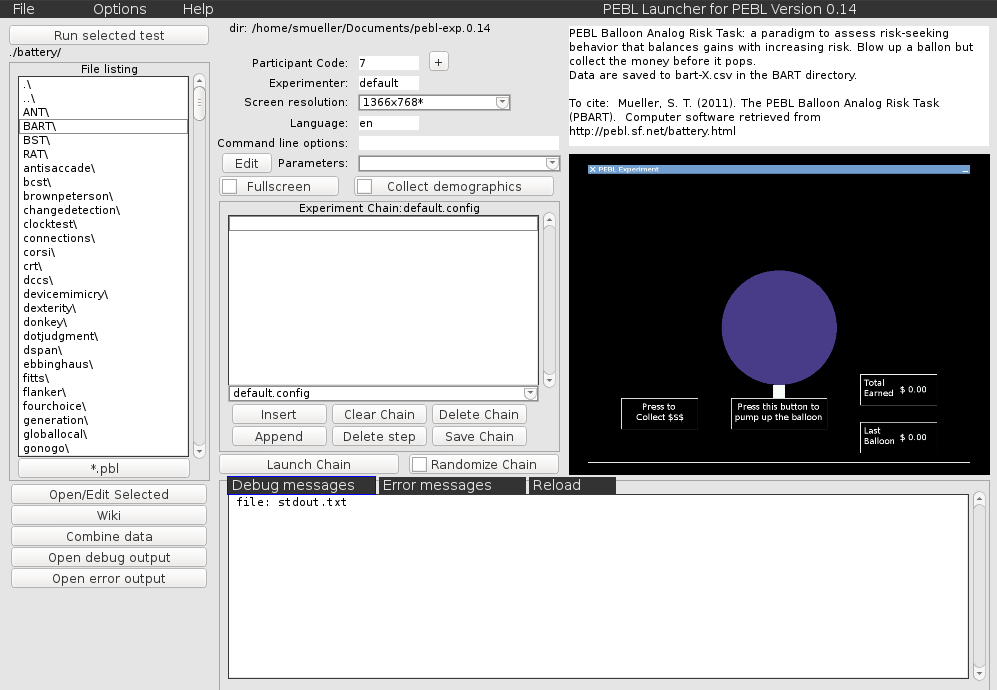
\includegraphics[scale=.35]{images/launcher.png} 
\end{figure}
\clearpage
\sect{History of the Launcher}
Prior to 2011, a front-end launcher was only available for PEBL on
Windows.  It was written in Visual Basic 6, which was old-fashioned,
single-platform, no longer supported by Microsoft, and created a
situation where a critical piece of PEBL infrastructure depended on a
non-free tool.  The main obstacle to a new launcher has always been:
PEBL needs a cross-platform launcher using a free software, and we
don't want to have to distribute a whole additional interpreter.  This
means that Python, wxBasic, TCL/TK, etc. were out of the
consideration.  Why couldn't there be an easy-to-use cross-platform
programming tool we could use?

As of PEBL Version 0.12, we found one: PEBL itself.  PEBL is not
really designed to create GUI applications, but it can be beat into
submission to do so.  For Version 0.12, enough filesystem access
functions and other features were available to make a reasonable
launcher.  

For PEBL 0.14, the launcher received a major overhaul.  With the advent of custom objects, we added a bunch of GUI objects (buttons, scrolling text boxes, checkboxes, menus, etc.) that enabled a much more polished version of the launcher that integrates better with other desktop options.  This allowed streamlining the launcher, adding functionality, improving its usefulness in the research lab. This includes the ability to set and change script-based parameters, which allows an experimenter to better tailor the PEBL battery tests to their particular needs.

\sect{How it works}
The simplest usage of the Launcher is that you use the file selector on
the left to choose a .pbl file, then click the button 'Run selected
script'' to run that experiment.  ONLY .pbl files and directories will
appear in the file window.
\clearpage
\sect{Features}

\begin{wrapfigure}{r}{0.5\textwidth}
 \vspace{-40pt}
  \begin{center}
    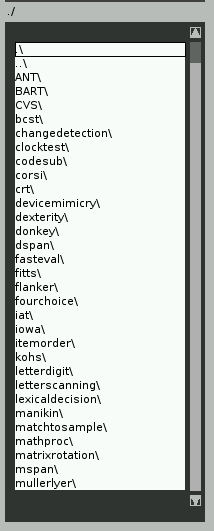
\includegraphics[scale=.5]{images/filebrowser.png} 
  \end{center}
  \caption{The File Browser.}
 \vspace{-40pt}
\end{wrapfigure}
\subsection{File browser}
On the left is a file browser.  It will only show .pbl files and
subdirectories.  To navigate to a subdirectory, simply click on the
directory to select it, then click on the selected directory.  To move
back up a directory, click on the '..\textbackslash' row.  When you have a .pbl file
selected, you can use the 'Run selected script' button to launch it.


\subsection{Participant code}
This will allow you to select the participant code you want sent to
any experiments you are about to run.  By default, PEBL saves the last
experiment code when you exit, and then reloads it the next time,
incrementing by one.  This makes it easier to avoid colliding
participant codes and overwriting data.  Participant code need not be
a number, but the launcher currently does not understand how to
increment non-numeric codes, and will probably restart at 1.  The plus button next to the 
code box will increment the current number by 1, which is useful if you are running multiple sessions in a row.

The automatic incrementation of participant code can be turned off by
opening the fileselect.pbl file and changing the variable gAutoSubcode
from 1 to 0.

When an experiment is launched, the specified code will be fed into
the experiment using the -s command-line option, and will be bound to
the gSubNum variable.  Some of the standard experiments will ask you
to enter a participant code regardless of whether you have one selected.
If that is the case, you should be able to edit the script to remove
the request to specify a participant code. However, most experiments in
the test battery should only ask the experimenter to specify a participant
code if the participant code is '0', which is what it will be when no -s
command is given.  So, if you are using code 0, many of the
experiments will ask you to enter a code after they launch.


\subsection{Experimenter code}
Many times, you may wish to keep track of the experimenter or research
assistant who collected the data.  Have them enter their name in the
'experimenter' window.  The name will be saved on exit.  The
experimenter code will be saved to the runlog file (see below). 

\subsection{Language}
Some experiments have instructions and stimuli that are translated
into different languages.  Enter your two-character language code in
the language box to tell the experiment what language to use. If your
chosen language is not available, the experiment will fall back to
English.  For Chinese and related languages, setting this will also change the default fontface used.  If you want to translate an experiment into your own
language, ask on the PEBL mailing list.



\subsection{Commmand Line Options}
There are a number of command line options available for PEBL that are not present as options in the launcher.  If you want to use any, you can type them in the ``Command line Options'' box and the launcher will pass them to PEBL.  You can use these to specify -V options that pass parameters into your experiment (e.g., controlling whether a practice or a test round is given).


\subsection{Edit and Parameters} The Edit button will let you edit the parameters used in the test.  When you edit and save the parameter set, it will then appear as an option in the parameters pulldown.  Before you run an experiment, you can select the parameter set you want to use from the pulldown (or save it permanently to an experiment chain).


\subsection{Fullscreen Mode}
If you want to launch your experiment in full-screen mode to improve
video latency and to avoid distractions, check this box. The secret
escape key combo is ctrl-alt-shift-\textbackslash : hit these four to abort out of
an experiment before it is complete.

\subsection{Demographics Collection}
The U.S. NIMH requires a number of demographic variables for research
they fund. Checking this box will collect this data and save it to a
data log file called demographics-log.csv, prior to running your experiment or experiment chain.

\subsection{Experiment Chains}
The launcher allows you to set up a 'chain' of experiments that get run in sequence.  All the experiments will be run consecutively, with an identical subject code.  This is accomplished by running a separate instance of PEBL for each experiment.  This can sometimes lead to a 'flash' between each experiment if running in fullscreen mode. 
Below the experiment chain window is a pulldown that lets you select the particular chain you want to use.  The default chain is loaded by default, and is also responsible for setting the parameter sets above.  

\subsection{Saving Experiment Chains}
When you exit the launcher, the current experiment chain will get saved in the the current config file.  By default, this file is called default.config.  This same file is loaded when the launcher starts again, restoring your settings.  By hitting the 'save chain' button, you will be asked to enter a new name to save the current configuration under.  Similarly, 'Delete chain' will delete the file in which the current chain is saved.  A chain can be loaded at start-up (by specifying the name of the config file with the -v command-line option). 

\subsection{Editing Experiment chains}  A chain can be edited by inserting, appending, or deleting steps, or clearing the entire chain, using the buttons below the experiment chain box.  Be sure to save the chain after editing so your edits will be saved.


\subsection{Loading Experiment Chains}
A previously saved experiment chain can be loaded by selecting the chain name from the pulldown selection box. 


\subsection{Description and Screenshot}
On the right side of the launcher is a window that will show a screenshot and print a description of a script when it is highlighted.  These need to be created by hand for each script.  The launcher does its best to show you a preview of the test inside any directory.  But to run an experiment, you need to select a .pbl file in the file window on the left. So, even if a screenshot appears on the right, you need to select the actual .pbl file to run the experiment.


\subsection{Message feedback windows}
Whenever a PEBL script runs, error and debug messages are saved to files called stdout.txt and stderr.txt, within the directory the file is run from.  When a test is completed, PEBL will look for and try to load these files in the tabbed window at the bottom of the launcher.  stdout.txt typically contains any messages saved using the Print() command, and is useful for debugging code. If an experiment crashes, it will be logged in the stderr.txt file and the Error messages tab.  In addition, a lot of  bookkeeping information is saved to that file, which can help diagnose other possible problems.  If you need to access these files directly to help report bugs, you can open them using the 'Open Debug Output'  and 'Open error output' buttons.

\

\subsection{Other buttons}
The launcher has a number of other buttons to help you use PEBL.
These include:
\begin{itemize}

\item \emph{Open/Edit selected} On the lower left, there is a button labeled ``Open/Edit selected''.  This
  will open a selected .pbl script in a text editor, and will open a
  directory in your system's file manager.  An easy way to look at or
  make changes to the script, or to locate data files after a script is run. 

\item \emph{Wiki} This will launch a web browser that will take you to the PEBL wiki page that is related to the currently selected test.  THis should help provide information about the test, its background, parameters, and data format.


\item\emph{Combine data} This will launch a data combining utility described below.  It will help merge all your data files together into a single spreadsheet.

\item \emph{Open debug output} Whenever an experiment is run, any time
  you use the Print() function, it will print the resulting text to a
  file names stdout.txt the directory it was run in.  This button will
  open that file.

\item \emph{Open error output} Whenever an experiment is run, the
  error and status messages are saved to a file called stderr.txt in
  the directory it was run in.  This button will open that file.


\end{itemize}

\subsection{Menu}
A lot of functionality is present in menus at the top of the window. 

\begin{itemize}
\item \emph{File|Exit} This will exit the launcher and save the current
  configuration options to the named experiment chain.
\item \emph{Options|change launcher size}. The launcher has trouble running on netbooks with only 600 pixels vertical distance.  This will make a 'small' launcher that is more compact, but only works next time the launcher is opened.

\item \emph{Help|About} This provides a short description of the launcher.

\item \emph{Help|Manual} This opens the PEBL .pdf manual.  The manual
  is located in different places on each platform, and will change
  names for each release.


\item \emph{Help|Website}  This will take you to the main PEBL website.

\item \emph{Help|Wiki} This button will take you to the PEBL wiki, and do
  its best to find a WIKI page related to the experiment you are
  looking at. They won't always exist, and if not, you can always sign
  in and make your own.

\item \emph{Help|Tutorial} This will open a wiki page containing a basic PEBL usage tutorial.

\item \emph{Help|Review} This will let you provide feedback about PEBL
\item \emph{Help|Donate} This will let you donate funds to help support PEBL development.

\end{itemize}

\sect{Launching an experiment}

To launch an experiment, navigate through the directories in the file listing box.  Only directories and files with the .pbl extension are shown in this box.  To open a directory, click once to move the highlight box onto the directory name, and a second time to open the directory.  When a new directory is opened, the first available .pbl file will be automatically selected.  To run that script, just press the 'Run Selected script' button above the file select box.  It will run with the specified parameter, including subject code, language, fullscreen mode.  In addition, if the 'collect demographics' button is selected, a demographic survey will happen prior to the study running.

\sect{Launching an experiment chain}
If you have a series of experiments you want to run, create an experiment chain and launch it using the 'Launch chain' button above the experiment chain selection box.  Tip: Use experiment chains even if you are are running just single experiment, with just a single experiment selected.  This give faster access and is less error-proned.

\sect{Translating the Launcher}
You can translate the launcher to your own language.  Open the launcher file (fileselect.pbl), and go to the end of the script, to a function named ``GetStrings'':
\begin{verbatim}
define GetStrings(lang)
{
   lang <- Uppercase(lang)
   if(lang == "EN")
   {
      gRunText <- "Run selected script"
      gOpenText <- "Open"
      gExitText <- "EXIT"
      gViewDebugText <- "View debug output"
      gViewErrorText <- "View error output"
      gAddToChainText <- "Add to Chain"
      gClearChainText <- "Clear Chain"
      gSaveChainText <- "Save Chain"
....
\end{verbatim}

The labels used in the launcher all appear here.  You should be able to just translate the text of each on into the language of your choice.  Send the translations back to the author so they can be incorporated into the next launcher version.  You can also make a section in the if statement for your particular language.  When you change the language in launcher, it will save that option and use your language of choice next time.

\sect{Utility:Parameter setting}
Version 0.14 of the PEBL Launcher allows you to set parameters from tests before launching.  A basic screenshot is shown below:


 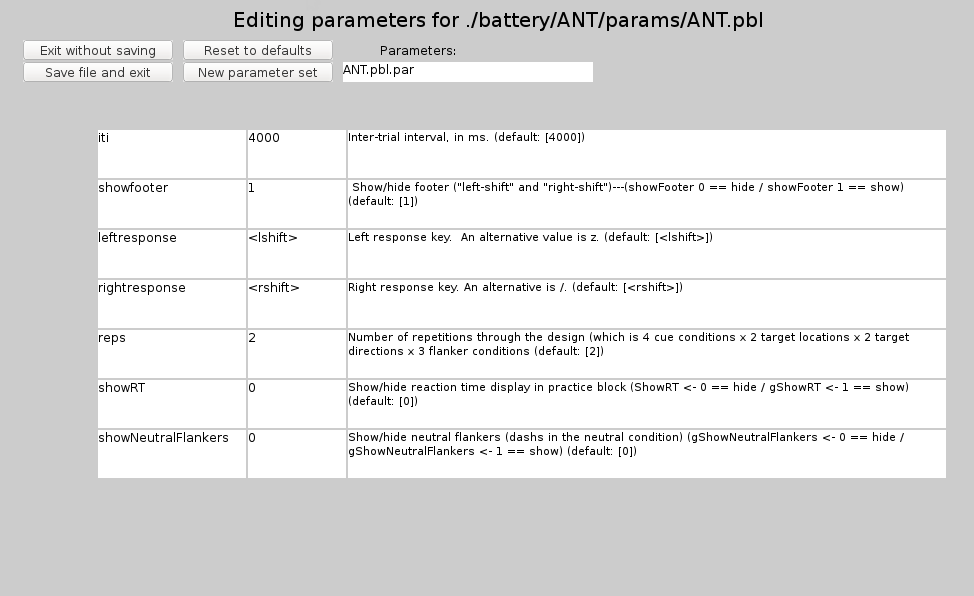
\includegraphics[scale=.3]{images/params.png} 
 
Here, the first column shows the name of the parameter. The second is the current value, which can be edited by clicking on the box and typing a new value.  When complete, hit enter and the new set will be recorded.  The rightmost column provides a basic description of the parameter, and its default value.  

To create a new parameter set, write the name of the parameter set you want to use in the box at the top of the screen. Then, when you hit 'Save file and exit', it will be saved to this parameter file. There is no need to include .par in the filename, as it will be added if you do not add it yourself.   To edit a current parameter set, select the parameter set you want and press 'edit' in the main window.
 
 
\sect{Utility: Combining data files}
Once an experiment is done, the data files are typically stored within the data directory in which the test appeared.  Furthermore, each participant may be saved in his or her own subdirectory. On some tests, a merged or pooled data file is also saved, but this is not always the case.  In order to merge all of you data into one master file, you can use PEBL's data combining tool, accessible through a button on the lower left of the 
launcher.

To use this, navigate to the data directory of your tests, and click the 'Combine data' button.  A screen like the one below should open.


 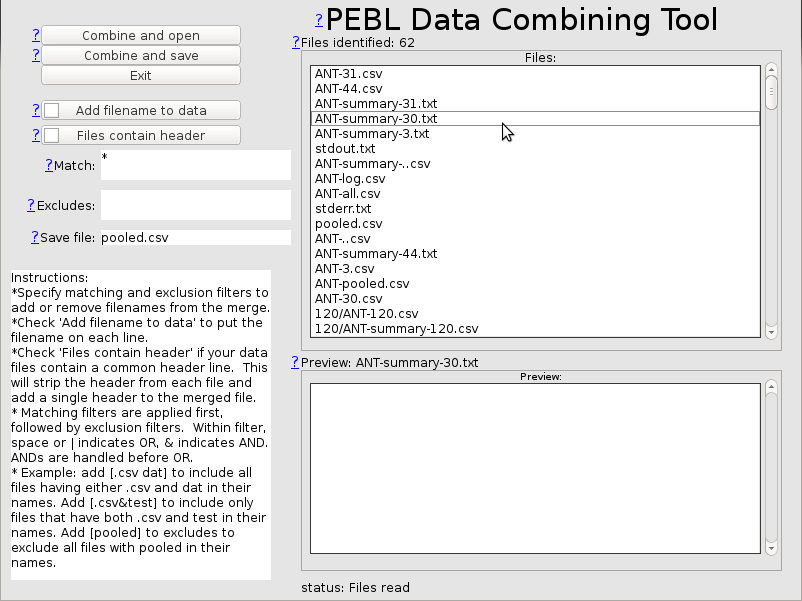
\includegraphics[scale=.4]{images/combine.png} 
  
On the upper right, a list of all files within the selected directory (and subdirectories) will be displayed.  You want to choose some (but probably not all) of these.  You can choose a subset by typing match values into the match and exclude boxes on the left.  Currently, the * indicates all files will match.  You may want to just include .csv files, in which case deleting the * and typing csv into the box will bring up only files with csv in their name.  You may want to exclude summary files, in which case you can type summary into the excludes box.  Each time you change the selection criteria and hit enter, the list of files will update.  A preview of any of the files can be seen in the lower right window.  IN the match and exclude boxes, spaces act as logical 'or's.  matching with the following '* csv' will match all files, because the first * will match all files. Or can also be specified using the | character.  The \& character can be used to specify AND criteria.  To match csv files from participant 300, you would enter '\texttt{300\&csv}'.  The matches are process before the excludes.

Once you have selected the right files using match and exclude criteria, you should determine whether the files have a header. If they have a header, you probably want to remove the header, including just once in the merged file. The combiner is not smart enough to detect this on its own, so you must check 'files contain header' if you want the header stripped from each individual data set and added to the final merged set.

Finally, especially if your data does not have a participant code in it, you may check 'add filename to data' which will add a column at the beginning of the data indicating the source file of each row of data.

Once you are ready, you can choose 'combine and save' which will save the data to the filename you specified in 'save file'.  If you use the combiner more than once, be sure to exclude 'pooled' from your match list so you don't get multiple copies of your data.  You can also choose 'combine and  open', which will create the pooled file, but then try to open in with whatever program is associated with that file type (i.e., microsoft excel for .csv files).

%%% Local Variables: 
%%% mode: latex
%%% TeX-master: "main"
%%% End: 
